\documentclass{include/protokollclass}
% Main File - Based on protokollclass.cls
% Comments are mostly in English (and some in German, concerning the Praktikum)
% ------------------------------------------------------------------------------
% Further files in folder:
%  - include/cmds.tex (for macros and additional commands)
%  - include/kitlogo.pdf (for titlepage)
%  - lit.bib (bibtex bibliography database)
%  - include/titlepage.tex (for layout of titelpage)
% ------------------------------------------------------------------------------
% Useful Supplied Packages:
% amsmath, amssymb, mathtools, bbm, upgreek, nicefrac,
% siunitx, varioref, booktabs, graphicx, tikz, multicol

\usepackage{rotating}
\usepackage{icomma}
\usepackage{subfig}
\usepackage{pdfpages}
\usepackage[onehalfspacing]{setspace}



%% ---------------------------------------------
%% |    Informationen über dieses Protokoll    |
%% ---------------------------------------------
\newcommand{\praktikum}{P1}                % P1 oder P2
\newcommand{\semester}{WS16/17}            % z.B. "WS14/15" oder "SS15"

\newcommand{\wochentag}{Di}                % Mo, Di, Mi oder Do
\newcommand{\gruppennr}{04}                % Zweistellige Gruppennummer

\newcommand{\nachnamea}{Friedrich}             % Nachname des ersten Praktikanten
\newcommand{\vornamea}{Tabea}               % Vorname des ersten Praktikanten
\newcommand{\nachnameb}{Stockmeier}              % Nachname des zweiten Praktikanten
\newcommand{\vornameb}{Lea}              % Vorname des zweiten Praktikanten

\newcommand{\emailadressen}{lea.stockmeier@web.de, tabea.friedrich@t-online.de}
% optionale Angabe von Emailadresse(n) für den Kontakt mit dem Betreuer

\newcommand{\versuch}{Seismik} % Name des Versuchs
\newcommand{\versuchsnr}{80}               % bitte die korrekte Nummer dem 
                                           % Arbeitsplatz am Versuchstag 
                                           % entnehmen
\newcommand{\fehlerrechnung}{Nein}         % Ob Fehlerrechnung im Versuch 
                                           % durchgeführt wurde oder nicht

\newcommand{\betreuer}{M. Mustermann}      % Name des zuständigen Betreuers
\newcommand{\durchgefuehrt}{01.09.16}      % Datum, an dem der Versuch 
                                           % durchgeführt wurde





%% --------------------------------------
%% |    Settings for Word Separation    |
%% --------------------------------------
% Help for separation:
% In German package the following hints are additionally available:
% "- = Additional separation
% "| = Suppress ligation and possible separation (e.g. Schaf"|fell)
% "~ = Hyphenation without separation (e.g. bergauf und "~ab)
% "= = Hyphenation with separation before and after
% "" = Separation without a hyphenation (e.g. und/""oder)

% Describe separation hints here:
\hyphenation
{
    über-nom-me-nen an-ge-ge-be-nen
    %Pro-to-koll-in-stan-zen
    %Ma-na-ge-ment  Netz-werk-ele-men-ten
    %Netz-werk Netz-werk-re-ser-vie-rung
    %Netz-werk-adap-ter Fein-ju-stier-ung
    %Da-ten-strom-spe-zi-fi-ka-tion Pa-ket-rumpf
    %Kon-troll-in-stanz
}





% um die Titelseite per PDF-reader auszufüllen. Vorgefertigte Daten
% können in Datei 'data.tex' modifiziert werden.
%\setboolean{forminput}{true}
% um die Anmerkungen zu den Textfeldern anzeigen zu lassen
%\setboolean{showannotations}{true}
% Erneuern der Seitenzahl in jedem Kapitel
%\setboolean{chapResetPageNumb}{true}
% Einbinden der Kapitelnummer in der Seitenzahl
%\setboolean{chapWiseNumb}{true}
% english or ngerman (new german für neue deutsche Rechtschreibung statt german)
\SelectLanguage{ngerman}

\title{Geophysikalische Geländeübungen \\ SS 2018 \\ Seismik}
\subtitle{Messgebiet A59/1 (Riedheim)}
\author{\\ Svenja Müller \\ mueller-svenja@gmx.net
\\ \\und\\ \\
Lea Stockmeier \\ lea.stockmeier@web.de \\ \\ \\
Betreuer: Vorname1 Nachname1 und Vorname2 Nachname2}
\date{\vfill\vfill\vfill \today}


%% -----------------------
%% |    Main Document    |
%% -----------------------
\begin{document}
    % Titlepage und ToC
    \FrontMatter

    \maketitle

    \begingroup \let\clearpage\relax    % in order to avoid listoffigures and
    \tableofcontents                    % listoftables on new pages
    \listoffigures
    \listoftables
    \endgroup
    %\cleardoublepage



    % Contents
    \MainMatter
    
%     \emptychapter[1]{Messprotokoll 1}{} % usage: \emptychapter[page displayed 
                                        %        in toc]{name of the chapter}
%     \pseudochapter[3]{Messprotokoll 2}  % usage: \pseudochapter[number of pages 
                                        %        added]{name of the chapter}
    
    \chapter{Einleitung}
    Bei der geophysikalischen Geländeübung 2018 führten wir am ersten Messtag, den 22.05., die Magnetik-Messungen durch. Das folgende Protokoll beschreibt die Theorie, Versuchsdurchführung, Auswertung und Fehlerdiskussion zu diesem Versuch.

Bei den Messungen und im Protokoll verfolgten wir folgende Fragestellungen: Die erste große Fragestellung ist, ob mit der Magnetik der Gang lokalisiert werden kann. Bei der Kartierung stellten wir uns die Frage, ob wir den Gang so gut lokalisieren können, dass wir uns daran die Lage der weiteren Profile überlegen können.
Bei den Profilen stellten wir uns dann die Frage, ob diese wirklich senkrecht zum Gang angelegt wurden. Dazu dient vor allem ein Profil, das extra schräg zum Gang gewählt wurde, um zu sehen, ob überhaupt ein Unterschied festgestellt werden kann. Die senkrechten Profile sollen zeigen, ob ein gemeinsames, alle Verläufe der Totalintensitäten erklärendes Modell gefunden werden kann. Die Messungen mit dem Fluxgate verfolgen die Fragestellung, ob dabei sinnvoll das Zweikreisverfahren angewendet werden kann. Die Vermessung eines vorbeifahrenden Traktors und der Umgebung der Basisstation dienten zur Abschätzung der während der Messung durch äußere Einflüsse auftretenden Fehler.
    
    \chapter{Theoretische Grundlagen}
    \section{kjgkjgr} %\cleardoublepage
    
    \chapter{Versuchsdurchführung}
    Es wurden auch schon am Tag des Versuchs Mitschriebe und Lageskizzen der Versuche angefertigt. Diese sind in Abbildung \ref{fig:Mitschrieb_erstes} bis \ref{fig:Mitschrieb_letztes} im Anhang. 

\section{Basisstation}

Zuerst wurde die Basisstation aufgebaut. Ihre Lage bezüglich des Messgebiets ist in Abbildung \ref{fig:LageBasis} zu sehen. Sie besteht aus einem Torsions-Magneto"|meter, das die Vertikalkomponente des Magnetfelds misst, und steht während des gesamten Versuchstags am gleichen Ort. Dadurch können zeitliche Variationen während der Versuche erkannt werden und die Messergebnisse eventuell um diese Variationen korrigiert werden. Würde eine solche Messung nicht durchgeführt werden, könnten zeitliche Variationen im Erdmagnetfeld fälschlicherweise als örtliche Anomalien interpretiert werden. Beim Aufbau des Torsions-Magnetometers musste besonders auf die genaue Horizontierung geachtet werden, damit auch wirklich nur die Vertikalkomponente des Erdmagnetfelds gemessen wurde.

\begin{figure}[!ht]
 \centering
 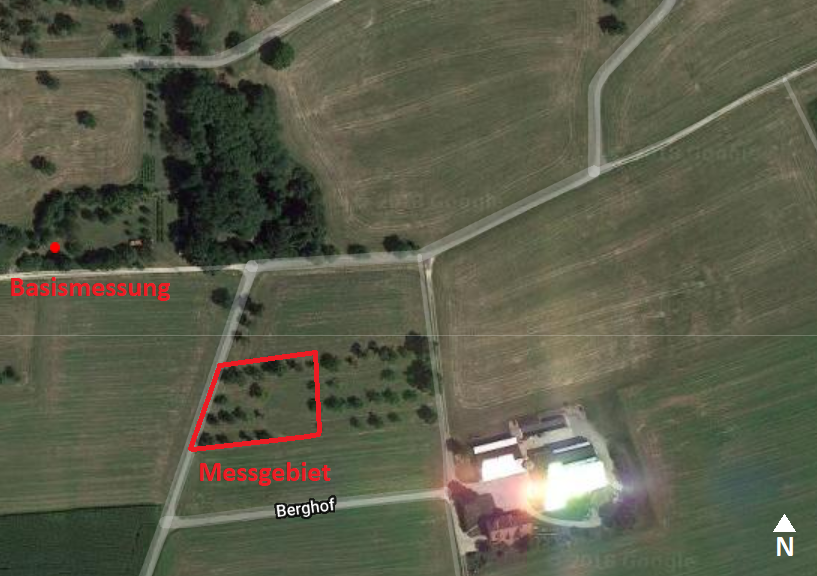
\includegraphics[width=0.5\textwidth]{fig/Basismessunggps}
 \caption[Lage der Basismessung und des Messgebiets]{Lage der Basismessung und des Messgebiets. Die Graphik wurde von Rebekka Kirchgässner und Luisa Rank übernommen.}
 \label{fig:LageBasis}
\end{figure}

Zuerst wurde das Torsions-Magnetometer kalibriert. Dazu wurde mit Hilfe eines Helmholtzspulenpaars ein über den Strom bekanntes Magnetfeld am Ort des Torsions-Magnetometers erzeugt. Durch eine lineare Regression kann in der Auswertung dann der Kalibrierungsfaktor $\frac{\tau}{|\vec{m}|}$ bestimmt werden.

Im Laufe des Tages wurde dann von 12:35 Uhr bis 17:17 Uhr alle 10 bis 20 Minuten ein Messwert an der Basisstation aufgenommen und Besonderheiten bei der Messung notiert. Beispielsweise war hin und wieder ein Traktor in der Nähe, von dem nicht klar war, ob er auf diese Entfernung schon  die Messung beeinflussen könnte. Das Torsions-Magnetometer musste auch einmal neu horizontiert werden.

\section{Kartierung}

Als nächstes wurde eine Kartierung mit einem Gradiometer durchgeführt. Um ein geeignetes Quadrat zur Durchführung dieser zu finden, wurde die Messwiese mit dem Gradiometer abgelaufen und Stellen mit großem Gradienten gesucht. So hatten wir bereits eine Idee, wo der Basaltgang verlaufen könnte. Außerdem entnahmen wir der geologischen Karte, in der der Basaltgang als magnetische Anomalie eingezeichnet ist, dass sich dieser ungefähr in Nord-Süd-Richtung vom Steinbruch, an dem der Gang an der Oberfläche aufgeschlossen ist, aus erstreckt.


Wir wählten dann das Quadrat M1-M2-M3-M4 mit einer Kantenlänge von 30 Metern, um die Kartierung durchzuführen. Das Quadrat befindet sich im in Abbildung \ref{fig:LageBasis} eingezeichneten Messgebiet. Dazu wurden Maßbänder entlang der Kanten möglichst senkrecht zueinander ausgelegt und dann mit möglichst gleichmäßiger Geschwindigkeit innerhalb von 30 Sekunden die Kante M1-M2 abgelaufen. Die Samplingrate in Laufrichtung betrug 8 Messungen pro Sekunde, also bei der richtigen Laufgeschwindigkeit auch 8 Messungen pro Meter. Dies wurde in 1\,Meter-Abständen 30 mal wiederholt (Skizze dazu siehe Abbildung \ref{fig:MessungKartierung}). Es ergibt sich also eine Kartierung auf diesem Quadrat aus insgesamt 720 Messpunkten.

\begin{figure}[!ht]
 \centering
 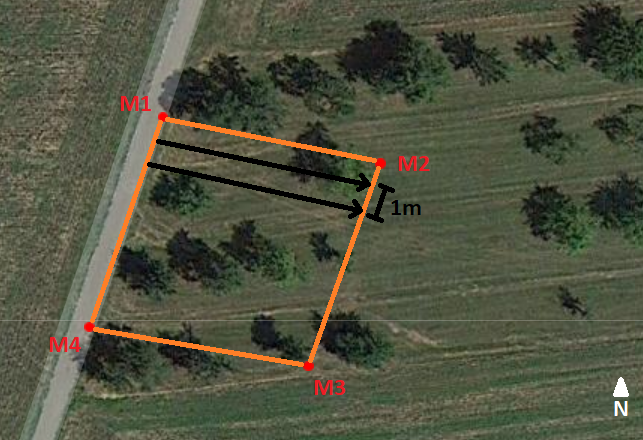
\includegraphics[width=0.5\textwidth]{fig/Kartierunggps}
 \caption[Durchführung der Kartierung]{Durchführung der Kartierung. Die Graphik wurde von Rebekka Kirchgässner und Luisa Rank übernommen.}
 \label{fig:MessungKartierung}
\end{figure}


% Zu Fehlerbetrachtungen????
Dabei auftretende Schwierigkeiten waren, dass manchmal ein Busch im Laufweg war und um diesen herumgelaufen werden musste. Außerdem fuhr einmal während der Messung ein Traktor vorbei. Eine weitere Schwierigkeit stellte die erforderliche gleichmäßige Geschwindigkeit dar. Nach der Hälfte wechselte die Beobachterin. Die zweite Beobachterin hatte nur einen Testlauf und auch bei den nächsten drei Bahnen kam sie manchmal ein bis zwei Sekunden zu früh oder spät am Ende des Quadrats an.

\section{Profile}

Nun musste bestimmt werden, entlang welcher Profile Messungen durchgeführt werden sollten. Dabei war entscheidend, dass die Software, mit welcher wir diese Messungen auswerten, von einer senkrechten Lage des Profils zum zu untersuchenden Objekt im Untergrund ausgeht.  Wir konnten bereits vor Ort das Ergebnis der Kartierung anschauen und wussten so, dass der Basaltgang parallel zur Diagonalen M1-M3 verläuft. Um dazu senkrecht zu messen, legten wir unsere Profile entlang der Diagonalen M4-M2 oder parallel zu dieser. Diese Profile nannten wir M22-M23, M21-M2 und M24-M25 (Lage siehe Abbildung \ref{fig:Profilegps}). Sie liegen im Abstand von zwei Metern nebeneinander. Das Profil M26-M27 ist auch senkrecht zum Gang angeordnet, aber aus dem Kartierungsergebnis zu schließen vermutlich nicht ganz mittig darüber. Um zu prüfen, ob an den Messergebnissen überhaupt zu erkennen ist, ob senkrecht oder in einem anderen Winkel zum Gang gemessen wurde, ist das Profil M28-M29 absichtlich schräg zum Gang angelegt worden. Ein weiteres Profil ohne Name verlief von der Basisstation aus am Tisch und der Hütte vorbei, um den Einfluss der Umgebung auf das Magnetfeld an der Basisstation zu untersuchen.

\begin{figure}[!ht]
 \centering
 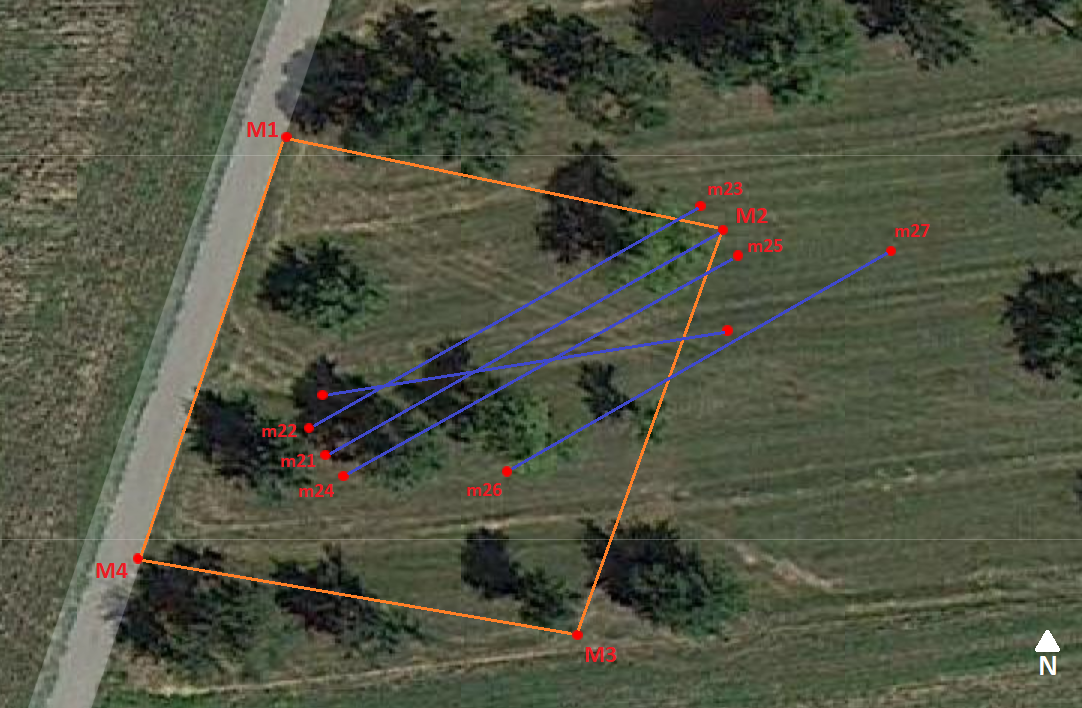
\includegraphics[width=0.8\textwidth]{fig/Profilegps}
 \caption[Lage der Profile bezüglich der Kartierung]{Lage der Profile bezüglich der Kartierung. Bei der Benennung der Profilenden sind Groß- und Kleinbuchstaben äquivalent. Die Graphik wurde von Rebekka Kirchgässner und Luisa Rank übernommen.}
 \label{fig:Profilegps}
\end{figure}

Alle Profile wurden mit einem der drei Protonen-Präzessions-Magnetometern ELSEC 1, ELSEC 2 und G-856 von Geometrics vermessen. Sie werden in diesem Protokoll nach ihren Nummern 1 und 2 bzw. neues Messgerät (G-856 von Geometrics) benannt. Die Profile M21-M2 und M24-M25 wurden außerdem mit einem Fluxgate-Magnetometer vermessen. Diese Messung diente dazu, auch dieses Messgerät kennenzulernen und eventuell das Zweikreisverfahren anwenden zu können.

\section{Vergleich der Messgeräte}

Am Ende des Versuchstags wurden mit jedem Protonen-Präzessions-Magnetometer vier Messungen am Ort der Basisstation durchgeführt. Auch mit dem Fluxgate-Magnetometer wurde eine Messung an der Basisstation durchgeführt. Diese Messung diente zur Überprüfung, ob die verschiedenen Magnetometer den gleichen Wert anzeigen. Falls dies nicht der Fall sein sollte, können dennoch die Messwerte dennoch verglichen werden, weil sie so auf den jeweiligen Wert an der Basisstation korrigiert werden können.
    
    \chapter{Auswertung}
    \section{Kalibrierung des Torsions-Magnetometers}

Die Messwerte der Kalibrierungsmessung sind in Abbildung \ref{fig:MPKalibrierung} zu sehen. Zur Auswertung wird zunächst der durch die Spulen fließende Strom mit dem Spulenkennwert $s$ und der Formel
\begin{equation}
 B=s\cdot I=I\cdot \eb{26,5}{nT}{mA} 
\end{equation}
in das Magnetfeld umgerechnet. Der Plot der Messwerte und der linearen Regression ist in Abbildung \ref{fig:kalibrierung} zu sehen. Bei der Regression ergab sich eine Steigung von $\eb{-0.0039}{Skt}{nT}$. Der negative Kehrwert dieser Steigung liefert den Kalibrierungsfaktor
\begin{equation}
 \frac{\tau}{|\vec{m}|}=\eb{253}{nT}{Skt} \fullstop
\end{equation}

\begin{figure}
 \centering
 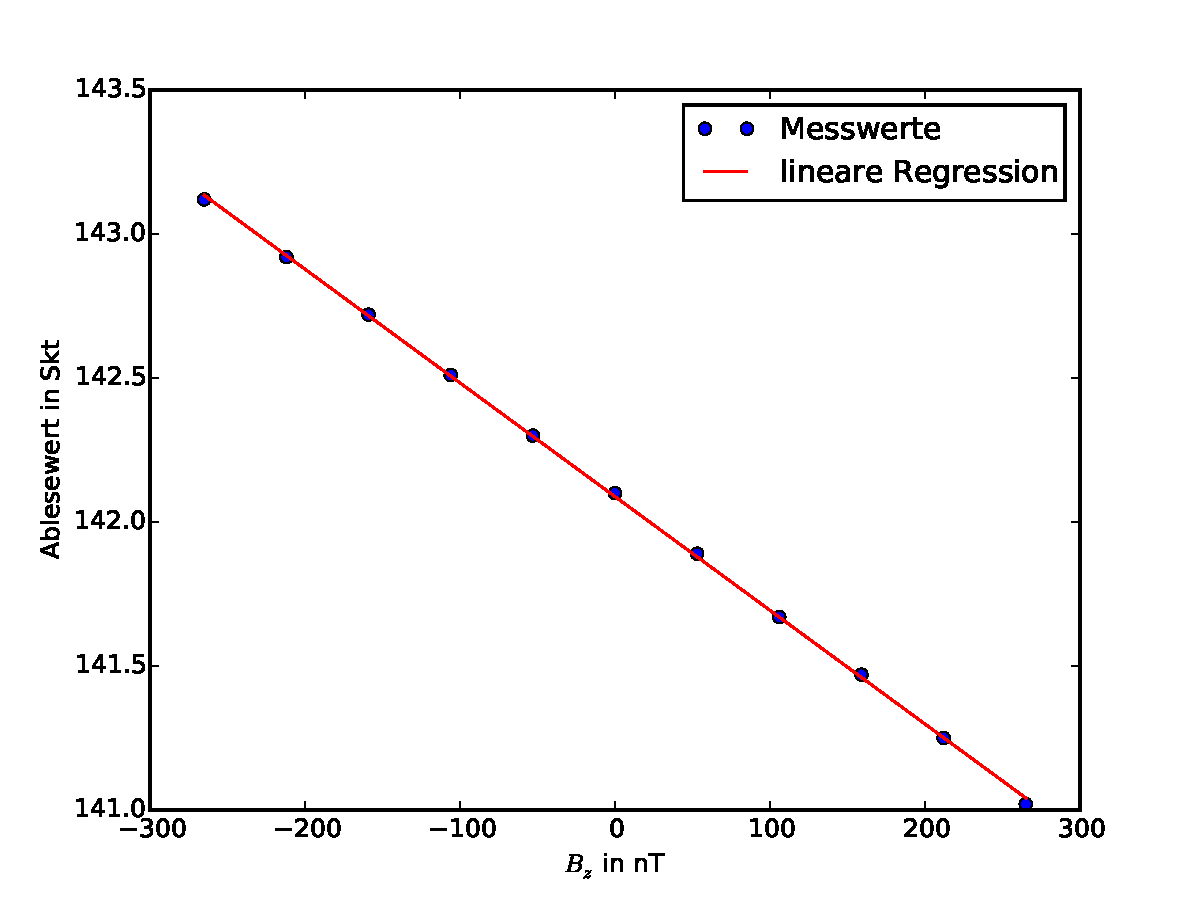
\includegraphics[width=\textwidth]{fig/kalibrierung.pdf}
 \caption[Bestimmung des Kalibrierungsfaktors des Torsions-Magnetometers]{Bestimmung des Kalibrierungsfaktors des Torsions-Magnetometers. Aufgetragen sind die Ablesewerte am Gfz in Skt über die angelegte magnetische Flussdichte in nT}
 \label{fig:kalibrierung}
\end{figure}


% \begin{figure}
%  \centering
%  \includegraphics[width=\textwidth]{fig/}
%  \caption{}
%  \label{fig:}
% \end{figure}

    % appendix for more or less interesting calculations
    \Appendix
    \chapter*{\appendixname} \addcontentsline{toc}{chapter}{\appendixname}
    % to make the appendix appear in ToC without number. \appendixname = 
    % Appendix or Anhang (depending on chosen language)
    \section{Messprotokolle}

\begin{figure}[h!]
 \centering
 \includegraphics[width=0.8\textwidth]{fig/Messprotokolle/Kalibrierung.png}
 \caption{Messprotokoll zur Kalibrierungsmessung}
 \label{fig:MPKalibrierung}
\end{figure}

\begin{figure}[h!]
 \centering
 \includegraphics[width=\textwidth]{fig/Messprotokolle/EinflussHuette.png}
 \caption{Messprotokoll zum Profil zur Untersuchung der Einflüsse äußerer Störfaktoren auf die Basismessung}
 \label{fig:MPHuette}
\end{figure}

% \begin{figure}[h!]
%  \centering
%  \includegraphics[width=\textwidth]{fig/Messprotokolle/}
%  \caption{}
%  \label{fig:}
% \end{figure} %\cleardoublepage



    % Bibliography
    \TheBibliography

    % BIBTEX
    % use if you want citations to appear even if they are not referenced to: 
    % \nocite{*} or maybe \nocite{Kon64,And59} for specific entries
    %\nocite{*}
    \bibliographystyle{babalpha}
    \bibliography{lit.bib}

    % THEBIBLIOGRAPHY
    %\begin{thebibliography}{000}
    %    \bibitem{ident}Entry into Bibliography.
    %\end{thebibliography}
\end{document}
